\documentclass[10pt]{article}
\usepackage{multirow}
\usepackage{spheric}
%%%TITLE
\title{Image processing with the SPH method}
\date{}

%%AFFILIATIONS
\author[1]{Chunying HUANG$^\dagger$}
\author[1]{Wenhuan LU}
\author[2]{Darcy Q. HOU}
\author[2]{Xin CHENG}

\affil[1]{School of Computer Software, Tianjin University, China}
\affil[2]{School of Computer Science and Technology, Tianjin University, China}
\affil[$\relax$]{\email{\dagger}{cyhuang416@163.com}}


%%DOCUMENT
\begin{document}

\maketitle

%\SelectedTopics{}

%%PLEASE PUT YOUR ABSTRACT HERE
\begin{abstract}
One of the most significant research fields in computer graphics is the digital image processing. Scaling, rotating and repairing are the fundamental components in image processing which are all based on interpolation. There are many grid-based interpolation algorithms for image processing such as the nearest neighbor interpolation, bilinear interpolation, polynomial interpolation, B-spline interpolation and cubic convolution interpolation \cite{parker1983comparison,carey1999regularity}. Although these algorithms have achieved great success, their dependence on the grids might introduce difficulties and disadvantages for advanced image processing. On the other hand, the meshless methods only use the image information in the support domain to compensate the missing parts without the limit of grids. In this paper, the meshless smoothed particle hydrodynamics (SPH) method and the corrective smoothed particle method (CSPM) are used to deal with scaling, rotating and repairing of three typical images including Lenna, Pepper and Stanford Dragon as shown in Fig. \ref{fig:fig:51}. The numerical results indicate that the meshless methods can obtain better results according to the Peak Signal to Noise Ratio (PSNR) as shown in Table \ref{tab:51}. Moreover, dissipation of moving images has also been successfully achieved by modelling it with a convection-diffusion process. 

\begin{figure}[!htb]
\begin{minipage}[t]{0.33\linewidth}
\centering
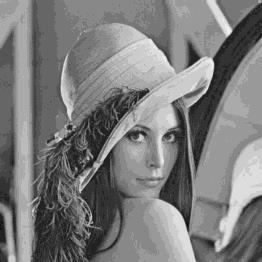
\includegraphics[width=0.8\textwidth]{51-1.png}\\
(a)
\end{minipage}
\begin{minipage}[t]{0.33\linewidth}
\centering
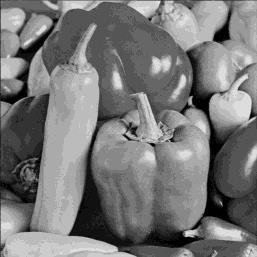
\includegraphics[width=0.8\textwidth]{51-2.png}\\
(b)
\end{minipage}
\begin{minipage}[t]{0.33\linewidth}
\centering
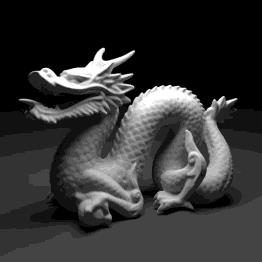
\includegraphics[width=0.8\textwidth]{51-3.png}\\
(c)
\end{minipage}
\caption{Typical images for processing}\label{fig:fig:51}
\end{figure}




\begin{table}[!htb]
\centering
\caption{PSNRs in scaling for different image interpolation methods}\label{tab:51}
\begin{tabular}{ccccc}
\hline 
\multirow{2}{*}{Case name} & \multicolumn{4}{c}{Interpolation methods}\tabularnewline
\cline{2-5} 
 & Nearest neighbor & Bilinear & SPH & CSPM\tabularnewline
\hline 
Lenna & 28.1987  & 28.1984 & 29.7391 & 31.1865\tabularnewline
Pepper & 27.1608 & 28.3115 & 30.7758 & 28.9502\tabularnewline
Standford Dragon & 28.5788 & 30.5884 & 31.7239 & 31.8727\tabularnewline
\hline 
\end{tabular}
\end{table}

\end{abstract}


%%THE END OF ABSTRACT

\addbib

\end{document}
